\documentclass[1p]{elsarticle_modified}
%\bibliographystyle{elsarticle-num}

%\usepackage[colorlinks]{hyperref}
%\usepackage{abbrmath_seonhwa} %\Abb, \Ascr, \Acal ,\Abf, \Afrak
\usepackage{amsfonts}
\usepackage{amssymb}
\usepackage{amsmath}
\usepackage{amsthm}
\usepackage{scalefnt}
\usepackage{amsbsy}
\usepackage{kotex}
\usepackage{caption}
\usepackage{subfig}
\usepackage{color}
\usepackage{graphicx}
\usepackage{xcolor} %% white, black, red, green, blue, cyan, magenta, yellow
\usepackage{float}
\usepackage{setspace}
\usepackage{hyperref}

\usepackage{tikz}
\usetikzlibrary{arrows}

\usepackage{multirow}
\usepackage{array} % fixed length table
\usepackage{hhline}

%%%%%%%%%%%%%%%%%%%%%
\makeatletter
\renewcommand*\env@matrix[1][\arraystretch]{%
	\edef\arraystretch{#1}%
	\hskip -\arraycolsep
	\let\@ifnextchar\new@ifnextchar
	\array{*\c@MaxMatrixCols c}}
\makeatother %https://tex.stackexchange.com/questions/14071/how-can-i-increase-the-line-spacing-in-a-matrix
%%%%%%%%%%%%%%%

\usepackage[normalem]{ulem}

\newcommand{\msout}[1]{\ifmmode\text{\sout{\ensuremath{#1}}}\else\sout{#1}\fi}
%SOURCE: \msout is \stkout macro in https://tex.stackexchange.com/questions/20609/strikeout-in-math-mode

\newcommand{\cancel}[1]{
	\ifmmode
	{\color{red}\msout{#1}}
	\else
	{\color{red}\sout{#1}}
	\fi
}

\newcommand{\add}[1]{
	{\color{blue}\uwave{#1}}
}

\newcommand{\replace}[2]{
	\ifmmode
	{\color{red}\msout{#1}}{\color{blue}\uwave{#2}}
	\else
	{\color{red}\sout{#1}}{\color{blue}\uwave{#2}}
	\fi
}

\newcommand{\Sol}{\mathcal{S}} %segment
\newcommand{\D}{D} %diagram
\newcommand{\A}{\mathcal{A}} %arc


%%%%%%%%%%%%%%%%%%%%%%%%%%%%%5 test

\def\sl{\operatorname{\textup{SL}}(2,\Cbb)}
\def\psl{\operatorname{\textup{PSL}}(2,\Cbb)}
\def\quan{\mkern 1mu \triangleright \mkern 1mu}

\theoremstyle{definition}
\newtheorem{thm}{Theorem}[section]
\newtheorem{prop}[thm]{Proposition}
\newtheorem{lem}[thm]{Lemma}
\newtheorem{ques}[thm]{Question}
\newtheorem{cor}[thm]{Corollary}
\newtheorem{defn}[thm]{Definition}
\newtheorem{exam}[thm]{Example}
\newtheorem{rmk}[thm]{Remark}
\newtheorem{alg}[thm]{Algorithm}

\newcommand{\I}{\sqrt{-1}}
\begin{document}

%\begin{frontmatter}
%
%\title{Boundary parabolic representations of knots up to 8 crossings}
%
%%% Group authors per affiliation:
%\author{Yunhi Cho} 
%\address{Department of Mathematics, University of Seoul, Seoul, Korea}
%\ead{yhcho@uos.ac.kr}
%
%
%\author{Seonhwa Kim} %\fnref{s_kim}}
%\address{Center for Geometry and Physics, Institute for Basic Science, Pohang, 37673, Korea}
%\ead{ryeona17@ibs.re.kr}
%
%\author{Hyuk Kim}
%\address{Department of Mathematical Sciences, Seoul National University, Seoul 08826, Korea}
%\ead{hyukkim@snu.ac.kr}
%
%\author{Seokbeom Yoon}
%\address{Department of Mathematical Sciences, Seoul National University, Seoul, 08826,  Korea}
%\ead{sbyoon15@snu.ac.kr}
%
%\begin{abstract}
%We find all boundary parabolic representation of knots up to 8 crossings.
%
%\end{abstract}
%\begin{keyword}
%    \MSC[2010] 57M25 
%\end{keyword}
%
%\end{frontmatter}

%\linenumbers
%\tableofcontents
%
\newcommand\colored[1]{\textcolor{white}{\rule[-0.35ex]{0.8em}{1.4ex}}\kern-0.8em\color{red} #1}%
%\newcommand\colored[1]{\textcolor{white}{ #1}\kern-2.17ex	\textcolor{white}{ #1}\kern-1.81ex	\textcolor{white}{ #1}\kern-2.15ex\color{red}#1	}

{\Large $\underline{11a_{43}~(K11a_{43})}$}

\setlength{\tabcolsep}{10pt}
\renewcommand{\arraystretch}{1.6}
\vspace{1cm}\begin{tabular}{m{100pt}>{\centering\arraybackslash}m{274pt}}
\multirow{5}{120pt}{
	\centering
	\includegraphics[width=112pt]{../../../GIT/diagram.site/Diagrams/png/292_11a_43.png}\\
\ \ \ A knot diagram\footnotemark}&
\allowdisplaybreaks
\textbf{Linearized knot diagam} \\
\cline{2-2}
 &
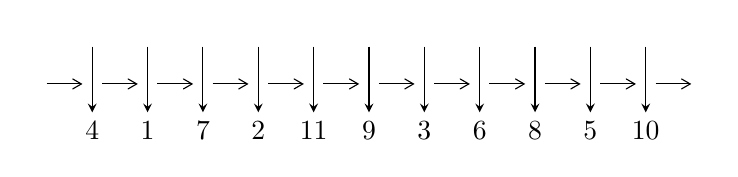
\begin{tikzpicture}[x=20pt, y=17pt]
	% nodes
	\node (C0) at (0, 0) {};
	\node (C1) at (1, 0) {};
	\node (C1U) at (1, +1) {};
	\node (C1D) at (1, -1) {4};

	\node (C2) at (2, 0) {};
	\node (C2U) at (2, +1) {};
	\node (C2D) at (2, -1) {1};

	\node (C3) at (3, 0) {};
	\node (C3U) at (3, +1) {};
	\node (C3D) at (3, -1) {7};

	\node (C4) at (4, 0) {};
	\node (C4U) at (4, +1) {};
	\node (C4D) at (4, -1) {2};

	\node (C5) at (5, 0) {};
	\node (C5U) at (5, +1) {};
	\node (C5D) at (5, -1) {11};

	\node (C6) at (6, 0) {};
	\node (C6U) at (6, +1) {};
	\node (C6D) at (6, -1) {9};

	\node (C7) at (7, 0) {};
	\node (C7U) at (7, +1) {};
	\node (C7D) at (7, -1) {3};

	\node (C8) at (8, 0) {};
	\node (C8U) at (8, +1) {};
	\node (C8D) at (8, -1) {6};

	\node (C9) at (9, 0) {};
	\node (C9U) at (9, +1) {};
	\node (C9D) at (9, -1) {8};

	\node (C10) at (10, 0) {};
	\node (C10U) at (10, +1) {};
	\node (C10D) at (10, -1) {5};

	\node (C11) at (11, 0) {};
	\node (C11U) at (11, +1) {};
	\node (C11D) at (11, -1) {10};
	\node (C12) at (12, 0) {};

	% arrows
	\draw[->,>={angle 60}]
	(C0) edge (C1) (C1) edge (C2) (C2) edge (C3) (C3) edge (C4) (C4) edge (C5) (C5) edge (C6) (C6) edge (C7) (C7) edge (C8) (C8) edge (C9) (C9) edge (C10) (C10) edge (C11) (C11) edge (C12) ;	\draw[->,>=stealth]
	(C1U) edge (C1D) (C2U) edge (C2D) (C3U) edge (C3D) (C4U) edge (C4D) (C5U) edge (C5D) (C6U) edge (C6D) (C7U) edge (C7D) (C8U) edge (C8D) (C9U) edge (C9D) (C10U) edge (C10D) (C11U) edge (C11D) ;
	\end{tikzpicture} \\
\hhline{~~} \\& 
\textbf{Solving Sequence} \\ \cline{2-2} 
 &
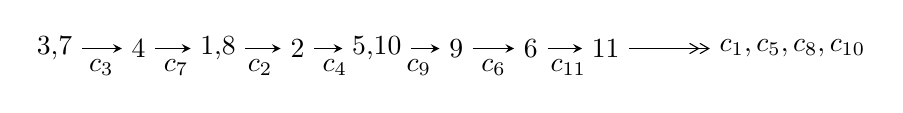
\begin{tikzpicture}[x=27pt, y=7pt]
	% node
	\node (A0) at (-1/8, 0) {3,7};
	\node (A1) at (1, 0) {4};
	\node (A2) at (33/16, 0) {1,8};
	\node (A3) at (25/8, 0) {2};
	\node (A4) at (67/16, 0) {5,10};
	\node (A5) at (21/4, 0) {9};
	\node (A6) at (25/4, 0) {6};
	\node (A7) at (29/4, 0) {11};
	\node (C1) at (1/2, -1) {$c_{3}$};
	\node (C2) at (3/2, -1) {$c_{7}$};
	\node (C3) at (21/8, -1) {$c_{2}$};
	\node (C4) at (29/8, -1) {$c_{4}$};
	\node (C5) at (19/4, -1) {$c_{9}$};
	\node (C6) at (23/4, -1) {$c_{6}$};
	\node (C7) at (27/4, -1) {$c_{11}$};
	\node (A8) at (39/4, 0) {$c_{1},c_{5},c_{8},c_{10}$};

	% edge
	\draw[->,>=stealth]	
	(A0) edge (A1) (A1) edge (A2) (A2) edge (A3) (A3) edge (A4) (A4) edge (A5) (A5) edge (A6) (A6) edge (A7) ;
	\draw[->>,>={angle 60}]	
	(A7) edge (A8);
\end{tikzpicture} \\ 

\end{tabular} \\

\footnotetext{
The image of knot diagram is generated by the software ``\textbf{Draw programme}" developed by Andrew Bartholomew(\url{http://www.layer8.co.uk/maths/draw/index.htm\#Running-draw}), where we modified some parts for our purpose(\url{https://github.com/CATsTAILs/LinksPainter}).
}\phantom \\ \newline 
\centering \textbf{Ideals for irreducible components\footnotemark of $X_{\text{par}}$} 
 
\begin{align*}
I^u_{1}&=\langle 
- u^9-2 u^8-3 u^7-2 u^6-3 u^5+2 u^4+2 u^3+4 u^2+4 d,\;u^9+u^8+u^7- u^6+u^5-3 u^4-2 u^3+4 c+4 u,\\
\phantom{I^u_{1}}&\phantom{= \langle  }- u^9-2 u^8-3 u^7-2 u^6- u^5+4 u^3+4 u^2+4 b,\;u^9+u^8+u^7- u^6- u^5-3 u^4-2 u^3-2 u^2+4 a+4 u,\\
\phantom{I^u_{1}}&\phantom{= \langle  }u^{11}+u^{10}+2 u^9+u^8+2 u^7-3 u^6-3 u^5-4 u^4-4 u^2+4 u+4\rangle \\
I^u_{2}&=\langle 
3 u^{15}+3 u^{14}+\cdots+4 d-4,\;2 u^{16}+u^{15}+\cdots+4 c+2,\\
\phantom{I^u_{2}}&\phantom{= \langle  }u^{14}+2 u^{12}+3 u^{10}+2 u^9+2 u^8+2 u^7+u^6+6 u^5+5 u^4+4 u^3+4 b+4,\;2 u^{15}+4 u^{14}+\cdots+4 a+10,\\
\phantom{I^u_{2}}&\phantom{= \langle  }u^{17}+2 u^{16}+\cdots-2 u-2\rangle \\
I^u_{3}&=\langle 
3 u^{15}+3 u^{14}+\cdots+4 d-4,\;2 u^{16}+u^{15}+\cdots+4 c+2,\\
\phantom{I^u_{3}}&\phantom{= \langle  }- u^{15}- u^{14}-3 u^{13}-2 u^{12}-5 u^{11}-3 u^{10}-7 u^9-2 u^8-5 u^7-3 u^6-10 u^5-11 u^4-7 u^3-2 u^2+4 b+2 u+4,\\
\phantom{I^u_{3}}&\phantom{= \langle  }-2 u^{16}-3 u^{15}+\cdots+4 a-2,\;u^{17}+2 u^{16}+\cdots-2 u-2\rangle \\
I^u_{4}&=\langle 
2 u^{16}+5 u^{15}+\cdots+4 d+14 u,\\
\phantom{I^u_{4}}&\phantom{= \langle  }- u^{15}-2 u^{13}-5 u^{11}-2 u^{10}-6 u^9-2 u^8-7 u^7-8 u^6-9 u^5-6 u^4-2 u^3-6 u^2+4 c-12 u-4,\\
\phantom{I^u_{4}}&\phantom{= \langle  }- u^{15}- u^{14}-3 u^{13}-2 u^{12}-5 u^{11}-3 u^{10}-7 u^9-2 u^8-5 u^7-3 u^6-10 u^5-11 u^4-7 u^3-2 u^2+4 b+2 u+4,\\
\phantom{I^u_{4}}&\phantom{= \langle  }-2 u^{16}-3 u^{15}+\cdots+4 a-2,\;u^{17}+2 u^{16}+\cdots-2 u-2\rangle \\
I^u_{5}&=\langle 
-2 a^2 c u+a^2 c+c a u+a^2 u-4 c a-2 c u- a^2+2 a u+2 d+5 c+a- u+1,\\
\phantom{I^u_{5}}&\phantom{= \langle  }a^2 c u+a^2 c-4 c a u- a^2 u+c^2+3 c a+2 c u+a u-2 c-3 a- u+2,\;- a^2 u+a^2- a u+b- a+2,\\
\phantom{I^u_{5}}&\phantom{= \langle  }a^3-2 a^2 u+3 a u- u,\;u^2- u+1\rangle \\
\\
I^v_{1}&=\langle 
a,\;d,\;c+1,\;b+1,\;v+1\rangle \\
I^v_{2}&=\langle 
c,\;d+1,\;b,\;a-1,\;v+1\rangle \\
I^v_{3}&=\langle 
a,\;d+1,\;c- a,\;b+1,\;v+1\rangle \\
I^v_{4}&=\langle 
a,\;d a+c+1,\;d v-1,\;c v+a+v,\;b+1\rangle \\
\end{align*}
\raggedright * 8 irreducible components of $\dim_{\mathbb{C}}=0$, with total 77 representations.\\
\raggedright * 1 irreducible components of $\dim_{\mathbb{C}}=1$ \\
\footnotetext{All coefficients of polynomials are rational numbers. But the coefficients are sometimes approximated in decimal forms when there is not enough margin.}
\newpage
\renewcommand{\arraystretch}{1}
\centering \section*{I. $I^u_{1}= \langle - u^9-2 u^8+\cdots+4 u^2+4 d,\;u^9+u^8+\cdots+4 c+4 u,\;- u^9-2 u^8+\cdots+4 u^2+4 b,\;u^9+u^8+\cdots+4 a+4 u,\;u^{11}+u^{10}+\cdots+4 u+4 \rangle$}
\flushleft \textbf{(i) Arc colorings}\\
\begin{tabular}{m{7pt} m{180pt} m{7pt} m{180pt} }
\flushright $a_{3}=$&$\begin{pmatrix}1\\0\end{pmatrix}$ \\
\flushright $a_{7}=$&$\begin{pmatrix}0\\u\end{pmatrix}$ \\
\flushright $a_{4}=$&$\begin{pmatrix}1\\u^2\end{pmatrix}$ \\
\flushright $a_{1}=$&$\begin{pmatrix}-\frac{1}{4} u^9-\frac{1}{4} u^8+\cdots+\frac{1}{2} u^2- u\\\frac{1}{4} u^9+\frac{1}{2} u^8+\cdots- u^3- u^2\end{pmatrix}$ \\
\flushright $a_{8}=$&$\begin{pmatrix}- u\\u\end{pmatrix}$ \\
\flushright $a_{2}=$&$\begin{pmatrix}-\frac{1}{4} u^9-\frac{1}{4} u^8+\cdots+\frac{1}{2} u^2+1\\\frac{1}{4} u^9+\frac{1}{4} u^7+\frac{1}{4} u^5\end{pmatrix}$ \\
\flushright $a_{5}=$&$\begin{pmatrix}\frac{1}{4} u^8+\frac{1}{2} u^7+\cdots-\frac{1}{2} u^2- u\\\frac{1}{4} u^{10}+\frac{1}{4} u^9+\cdots-\frac{1}{2} u^4+u^2\end{pmatrix}$ \\
\flushright $a_{10}=$&$\begin{pmatrix}-\frac{1}{4} u^9-\frac{1}{4} u^8+\cdots+\frac{1}{2} u^3- u\\\frac{1}{4} u^9+\frac{1}{2} u^8+\cdots-\frac{1}{2} u^3- u^2\end{pmatrix}$ \\
\flushright $a_{9}=$&$\begin{pmatrix}\frac{1}{4} u^{10}+\frac{1}{4} u^9+\cdots-\frac{1}{2} u^3- u\\-\frac{1}{4} u^{10}-\frac{1}{4} u^9+\cdots+\frac{1}{2} u^3- u^2\end{pmatrix}$ \\
\flushright $a_{6}=$&$\begin{pmatrix}-\frac{1}{4} u^8-\frac{1}{2} u^7+\cdots+u^2+u\\-\frac{1}{4} u^{10}-\frac{1}{4} u^9+\cdots+\frac{1}{2} u^3- u^2\end{pmatrix}$ \\
\flushright $a_{11}=$&$\begin{pmatrix}\frac{1}{2} u^6+\frac{1}{2} u^4+\frac{1}{2} u^2- u\\\frac{1}{2} u^8+\frac{1}{2} u^7+\cdots-\frac{1}{2} u^3- u^2\end{pmatrix}$\\ \flushright $a_{11}=$&$\begin{pmatrix}\frac{1}{2} u^6+\frac{1}{2} u^4+\frac{1}{2} u^2- u\\\frac{1}{2} u^8+\frac{1}{2} u^7+\cdots-\frac{1}{2} u^3- u^2\end{pmatrix}$\\&\end{tabular}
\flushleft \textbf{(ii) Obstruction class $= -1$}\\~\\
\flushleft \textbf{(iii) Cusp Shapes $= - u^{10}-3 u^9-4 u^8-5 u^7-4 u^6- u^5+3 u^4+4 u^3+2 u^2+4 u-10$}\\~\\
\newpage\renewcommand{\arraystretch}{1}
\flushleft \textbf{(iv) u-Polynomials at the component}\newline \\
\begin{tabular}{m{50pt}|m{274pt}}
Crossings & \hspace{64pt}u-Polynomials at each crossing \\
\hline $$\begin{aligned}c_{1},c_{4},c_{5}\\c_{6},c_{8},c_{10}\end{aligned}$$&$\begin{aligned}
&u^{11}- u^{10}-2 u^9+3 u^8+3 u^7-5 u^6+4 u^4-2 u^2+2 u+1
\end{aligned}$\\
\hline $$\begin{aligned}c_{2},c_{9},c_{11}\end{aligned}$$&$\begin{aligned}
&u^{11}+5 u^{10}+\cdots+8 u+1
\end{aligned}$\\
\hline $$\begin{aligned}c_{3},c_{7}\end{aligned}$$&$\begin{aligned}
&u^{11}+u^{10}+2 u^9+u^8+2 u^7-3 u^6-3 u^5-4 u^4-4 u^2+4 u+4
\end{aligned}$\\
\hline
\end{tabular}\\~\\
\newpage\renewcommand{\arraystretch}{1}
\flushleft \textbf{(v) Riley Polynomials at the component}\newline \\
\begin{tabular}{m{50pt}|m{274pt}}
Crossings & \hspace{64pt}Riley Polynomials at each crossing \\
\hline $$\begin{aligned}c_{1},c_{4},c_{5}\\c_{6},c_{8},c_{10}\end{aligned}$$&$\begin{aligned}
&y^{11}-5 y^{10}+\cdots+8 y-1
\end{aligned}$\\
\hline $$\begin{aligned}c_{2},c_{9},c_{11}\end{aligned}$$&$\begin{aligned}
&y^{11}+7 y^{10}+\cdots+40 y-1
\end{aligned}$\\
\hline $$\begin{aligned}c_{3},c_{7}\end{aligned}$$&$\begin{aligned}
&y^{11}+3 y^{10}+\cdots+48 y-16
\end{aligned}$\\
\hline
\end{tabular}\\~\\
\newpage\flushleft \textbf{(vi) Complex Volumes and Cusp Shapes}
$$\begin{array}{c|c|c}  
\text{Solutions to }I^u_{1}& \I (\text{vol} + \sqrt{-1}CS) & \text{Cusp shape}\\
 \hline 
\begin{aligned}
u &= \phantom{-}0.981646 + 0.091031 I \\
a &= \phantom{-}0.527474 + 0.160953 I \\
b &= -0.259189 + 0.777251 I \\
c &= -0.366942 - 0.136098 I \\
d &= \phantom{-}0.177956 + 0.945407 I\end{aligned}
 & -0.38453 + 3.51380 I & -10.33478 - 7.33311 I \\ \hline\begin{aligned}
u &= \phantom{-}0.981646 - 0.091031 I \\
a &= \phantom{-}0.527474 - 0.160953 I \\
b &= -0.259189 - 0.777251 I \\
c &= -0.366942 + 0.136098 I \\
d &= \phantom{-}0.177956 - 0.945407 I\end{aligned}
 & -0.38453 - 3.51380 I & -10.33478 + 7.33311 I \\ \hline\begin{aligned}
u &= \phantom{-}0.360685 + 1.114550 I \\
a &= \phantom{-}0.621176 - 0.836924 I \\
b &= \phantom{-}0.410237 + 0.659760 I \\
c &= \phantom{-}0.074184 - 1.245440 I \\
d &= \phantom{-}0.569474 + 1.085660 I\end{aligned}
 & \phantom{-}3.72768 - 0.41249 I & -4.65663 - 1.55838 I \\ \hline\begin{aligned}
u &= \phantom{-}0.360685 - 1.114550 I \\
a &= \phantom{-}0.621176 + 0.836924 I \\
b &= \phantom{-}0.410237 - 0.659760 I \\
c &= \phantom{-}0.074184 + 1.245440 I \\
d &= \phantom{-}0.569474 - 1.085660 I\end{aligned}
 & \phantom{-}3.72768 + 0.41249 I & -4.65663 + 1.55838 I \\ \hline\begin{aligned}
u &= -1.053240 + 0.696446 I \\
a &= \phantom{-}0.436462 - 0.109397 I \\
b &= -1.04374 - 1.24892 I \\
c &= -1.44166 + 0.27329 I \\
d &= \phantom{-}1.58561 + 1.00769 I\end{aligned}
 & -5.36867 - 9.54355 I & -15.3185 + 7.2879 I \\ \hline\begin{aligned}
u &= -1.053240 - 0.696446 I \\
a &= \phantom{-}0.436462 + 0.109397 I \\
b &= -1.04374 + 1.24892 I \\
c &= -1.44166 - 0.27329 I \\
d &= \phantom{-}1.58561 - 1.00769 I\end{aligned}
 & -5.36867 + 9.54355 I & -15.3185 - 7.2879 I\\
 \hline 
 \end{array}$$\newpage$$\begin{array}{c|c|c}  
\text{Solutions to }I^u_{1}& \I (\text{vol} + \sqrt{-1}CS) & \text{Cusp shape}\\
 \hline 
\begin{aligned}
u &= \phantom{-}0.306817 + 1.268500 I \\
a &= \phantom{-}0.136985 + 1.403680 I \\
b &= -0.369008 - 1.314180 I \\
c &= -0.860509 + 0.304947 I \\
d &= -0.184720 - 0.266859 I\end{aligned}
 & \phantom{-}3.91373 - 8.22510 I & -8.34823 + 8.49377 I \\ \hline\begin{aligned}
u &= \phantom{-}0.306817 - 1.268500 I \\
a &= \phantom{-}0.136985 - 1.403680 I \\
b &= -0.369008 + 1.314180 I \\
c &= -0.860509 - 0.304947 I \\
d &= -0.184720 + 0.266859 I\end{aligned}
 & \phantom{-}3.91373 + 8.22510 I & -8.34823 - 8.49377 I \\ \hline\begin{aligned}
u &= -0.809328 + 1.127750 I \\
a &= -0.58283 - 1.50488 I \\
b &= -1.16377 + 1.41429 I \\
c &= -0.19914 + 1.98351 I \\
d &= \phantom{-}1.51573 - 1.89641 I\end{aligned}
 & -3.9531 + 16.3093 I & -14.3050 - 10.3392 I \\ \hline\begin{aligned}
u &= -0.809328 - 1.127750 I \\
a &= -0.58283 + 1.50488 I \\
b &= -1.16377 - 1.41429 I \\
c &= -0.19914 - 1.98351 I \\
d &= \phantom{-}1.51573 + 1.89641 I\end{aligned}
 & -3.9531 - 16.3093 I & -14.3050 + 10.3392 I \\ \hline\begin{aligned}
u &= -0.573171\phantom{ +0.000000I} \\
a &= \phantom{-}0.721466\phantom{ +0.000000I} \\
b &= -0.149048\phantom{ +0.000000I} \\
c &= \phantom{-}0.588134\phantom{ +0.000000I} \\
d &= -0.328093\phantom{ +0.000000I}\end{aligned}
 & -0.805061\phantom{ +0.000000I} & -12.0740\phantom{ +0.000000I}\\
 \hline 
 \end{array}$$\newpage\newpage\renewcommand{\arraystretch}{1}
\centering \section*{II. $I^u_{2}= \langle 3 u^{15}+3 u^{14}+\cdots+4 d-4,\;2 u^{16}+u^{15}+\cdots+4 c+2,\;u^{14}+2 u^{12}+\cdots+4 b+4,\;2 u^{15}+4 u^{14}+\cdots+4 a+10,\;u^{17}+2 u^{16}+\cdots-2 u-2 \rangle$}
\flushleft \textbf{(i) Arc colorings}\\
\begin{tabular}{m{7pt} m{180pt} m{7pt} m{180pt} }
\flushright $a_{3}=$&$\begin{pmatrix}1\\0\end{pmatrix}$ \\
\flushright $a_{7}=$&$\begin{pmatrix}0\\u\end{pmatrix}$ \\
\flushright $a_{4}=$&$\begin{pmatrix}1\\u^2\end{pmatrix}$ \\
\flushright $a_{1}=$&$\begin{pmatrix}-\frac{1}{2} u^{15}- u^{14}+\cdots-7 u-\frac{5}{2}\\-\frac{1}{4} u^{14}-\frac{1}{2} u^{12}+\cdots- u^3-1\end{pmatrix}$ \\
\flushright $a_{8}=$&$\begin{pmatrix}- u\\u\end{pmatrix}$ \\
\flushright $a_{2}=$&$\begin{pmatrix}-\frac{1}{2} u^{15}- u^{14}+\cdots-8 u-\frac{5}{2}\\-\frac{3}{4} u^{14}-\frac{3}{2} u^{12}+\cdots-2 u^3-1\end{pmatrix}$ \\
\flushright $a_{5}=$&$\begin{pmatrix}-\frac{1}{2} u^{15}-\frac{5}{4} u^{14}+\cdots-7 u-\frac{7}{2}\\-\frac{1}{4} u^{16}-\frac{1}{2} u^{14}+\cdots-3 u^2- u\end{pmatrix}$ \\
\flushright $a_{10}=$&$\begin{pmatrix}-\frac{1}{2} u^{16}-\frac{1}{4} u^{15}+\cdots-\frac{1}{2} u-\frac{1}{2}\\-\frac{3}{4} u^{15}-\frac{3}{4} u^{14}+\cdots+\frac{1}{2} u+1\end{pmatrix}$ \\
\flushright $a_{9}=$&$\begin{pmatrix}-\frac{1}{4} u^{16}-\frac{3}{4} u^{14}+\cdots-\frac{3}{2} u-\frac{1}{2}\\-\frac{1}{4} u^{16}- u^{15}+\cdots+\frac{3}{2} u+1\end{pmatrix}$ \\
\flushright $a_{6}=$&$\begin{pmatrix}\frac{1}{2} u^{16}+u^{15}+\cdots+\frac{11}{4} u^2-\frac{1}{2}\\-\frac{1}{4} u^{16}- u^{15}+\cdots+\frac{3}{2} u+1\end{pmatrix}$ \\
\flushright $a_{11}=$&$\begin{pmatrix}-\frac{1}{2} u^{15}- u^{14}+\cdots-\frac{15}{2} u-3\\-\frac{1}{2} u^{14}- u^{12}+\cdots- u^3-1\end{pmatrix}$\\ \flushright $a_{11}=$&$\begin{pmatrix}-\frac{1}{2} u^{15}- u^{14}+\cdots-\frac{15}{2} u-3\\-\frac{1}{2} u^{14}- u^{12}+\cdots- u^3-1\end{pmatrix}$\\&\end{tabular}
\flushleft \textbf{(ii) Obstruction class $= -1$}\\~\\
\flushleft \textbf{(iii) Cusp Shapes $= 2 u^{16}+4 u^{15}+6 u^{14}+8 u^{13}+8 u^{12}+14 u^{11}+10 u^{10}+12 u^9+4 u^8+10 u^7+20 u^6+26 u^5+16 u^4-4 u^3-10 u^2-8 u-16$}\\~\\
\newpage\renewcommand{\arraystretch}{1}
\flushleft \textbf{(iv) u-Polynomials at the component}\newline \\
\begin{tabular}{m{50pt}|m{274pt}}
Crossings & \hspace{64pt}u-Polynomials at each crossing \\
\hline $$\begin{aligned}c_{1},c_{4}\end{aligned}$$&$\begin{aligned}
&u^{17}-5 u^{15}+\cdots+3 u^2-4
\end{aligned}$\\
\hline $$\begin{aligned}c_{2}\end{aligned}$$&$\begin{aligned}
&u^{17}+10 u^{16}+\cdots+24 u+16
\end{aligned}$\\
\hline $$\begin{aligned}c_{3},c_{7}\end{aligned}$$&$\begin{aligned}
&u^{17}+2 u^{16}+\cdots-2 u-2
\end{aligned}$\\
\hline $$\begin{aligned}c_{5},c_{6},c_{8}\\c_{10}\end{aligned}$$&$\begin{aligned}
&u^{17}-2 u^{16}+\cdots- u+1
\end{aligned}$\\
\hline $$\begin{aligned}c_{9},c_{11}\end{aligned}$$&$\begin{aligned}
&u^{17}+8 u^{16}+\cdots+3 u+1
\end{aligned}$\\
\hline
\end{tabular}\\~\\
\newpage\renewcommand{\arraystretch}{1}
\flushleft \textbf{(v) Riley Polynomials at the component}\newline \\
\begin{tabular}{m{50pt}|m{274pt}}
Crossings & \hspace{64pt}Riley Polynomials at each crossing \\
\hline $$\begin{aligned}c_{1},c_{4}\end{aligned}$$&$\begin{aligned}
&y^{17}-10 y^{16}+\cdots+24 y-16
\end{aligned}$\\
\hline $$\begin{aligned}c_{2}\end{aligned}$$&$\begin{aligned}
&y^{17}-10 y^{16}+\cdots+800 y-256
\end{aligned}$\\
\hline $$\begin{aligned}c_{3},c_{7}\end{aligned}$$&$\begin{aligned}
&y^{17}+6 y^{16}+\cdots+8 y-4
\end{aligned}$\\
\hline $$\begin{aligned}c_{5},c_{6},c_{8}\\c_{10}\end{aligned}$$&$\begin{aligned}
&y^{17}-8 y^{16}+\cdots+3 y-1
\end{aligned}$\\
\hline $$\begin{aligned}c_{9},c_{11}\end{aligned}$$&$\begin{aligned}
&y^{17}+4 y^{16}+\cdots-13 y-1
\end{aligned}$\\
\hline
\end{tabular}\\~\\
\newpage\flushleft \textbf{(vi) Complex Volumes and Cusp Shapes}
$$\begin{array}{c|c|c}  
\text{Solutions to }I^u_{2}& \I (\text{vol} + \sqrt{-1}CS) & \text{Cusp shape}\\
 \hline 
\begin{aligned}
u &= -0.742615 + 0.650908 I \\
a &= -1.40070 - 2.38570 I \\
b &= -1.30236 + 0.73752 I \\
c &= -0.757942 + 1.169930 I \\
d &= \phantom{-}1.088610 + 0.211420 I\end{aligned}
 & -6.94910 - 1.22724 I & -18.1485 + 0.8551 I \\ \hline\begin{aligned}
u &= -0.742615 - 0.650908 I \\
a &= -1.40070 + 2.38570 I \\
b &= -1.30236 - 0.73752 I \\
c &= -0.757942 - 1.169930 I \\
d &= \phantom{-}1.088610 - 0.211420 I\end{aligned}
 & -6.94910 + 1.22724 I & -18.1485 - 0.8551 I \\ \hline\begin{aligned}
u &= -0.834865 + 0.265014 I \\
a &= \phantom{-}0.511597 - 0.109110 I \\
b &= -0.597254 - 0.693509 I \\
c &= \phantom{-}0.800041 - 0.146031 I \\
d &= -0.807482 - 0.323646 I\end{aligned}
 & -0.670307 - 0.433874 I & -9.43166 - 0.87540 I \\ \hline\begin{aligned}
u &= -0.834865 - 0.265014 I \\
a &= \phantom{-}0.511597 + 0.109110 I \\
b &= -0.597254 + 0.693509 I \\
c &= \phantom{-}0.800041 + 0.146031 I \\
d &= -0.807482 + 0.323646 I\end{aligned}
 & -0.670307 + 0.433874 I & -9.43166 + 0.87540 I \\ \hline\begin{aligned}
u &= \phantom{-}0.976738 + 0.562668 I \\
a &= \phantom{-}0.583366 - 0.363840 I \\
b &= \phantom{-}0.537642 - 0.360420 I \\
c &= \phantom{-}0.879539 + 0.321552 I \\
d &= -1.09988 + 0.90044 I\end{aligned}
 & -2.67943 + 4.64771 I & -12.43915 - 4.11695 I \\ \hline\begin{aligned}
u &= \phantom{-}0.976738 - 0.562668 I \\
a &= \phantom{-}0.583366 + 0.363840 I \\
b &= \phantom{-}0.537642 + 0.360420 I \\
c &= \phantom{-}0.879539 - 0.321552 I \\
d &= -1.09988 - 0.90044 I\end{aligned}
 & -2.67943 - 4.64771 I & -12.43915 + 4.11695 I\\
 \hline 
 \end{array}$$\newpage$$\begin{array}{c|c|c}  
\text{Solutions to }I^u_{2}& \I (\text{vol} + \sqrt{-1}CS) & \text{Cusp shape}\\
 \hline 
\begin{aligned}
u &= -0.003992 + 0.842342 I \\
a &= \phantom{-}0.444102 - 0.000358 I \\
b &= -1.56684 - 0.00455 I \\
c &= \phantom{-}0.054218 - 0.565099 I \\
d &= -0.672214 + 0.818183 I\end{aligned}
 & -1.98005 - 1.46955 I & -8.36417 + 4.66528 I \\ \hline\begin{aligned}
u &= -0.003992 - 0.842342 I \\
a &= \phantom{-}0.444102 + 0.000358 I \\
b &= -1.56684 + 0.00455 I \\
c &= \phantom{-}0.054218 + 0.565099 I \\
d &= -0.672214 - 0.818183 I\end{aligned}
 & -1.98005 + 1.46955 I & -8.36417 - 4.66528 I \\ \hline\begin{aligned}
u &= -0.656745 + 1.004700 I \\
a &= \phantom{-}0.422901 - 0.058229 I \\
b &= -1.64195 - 0.84395 I \\
c &= -0.374228 + 1.227350 I \\
d &= \phantom{-}1.64609 - 1.04829 I\end{aligned}
 & -5.86965 + 6.57063 I & -15.2601 - 6.4345 I \\ \hline\begin{aligned}
u &= -0.656745 - 1.004700 I \\
a &= \phantom{-}0.422901 + 0.058229 I \\
b &= -1.64195 + 0.84395 I \\
c &= -0.374228 - 1.227350 I \\
d &= \phantom{-}1.64609 + 1.04829 I\end{aligned}
 & -5.86965 - 6.57063 I & -15.2601 + 6.4345 I \\ \hline\begin{aligned}
u &= -0.110097 + 1.246510 I \\
a &= \phantom{-}0.487558 + 1.065780 I \\
b &= \phantom{-}0.185932 - 1.001000 I \\
c &= \phantom{-}0.792244 - 0.317990 I \\
d &= \phantom{-}0.132799 + 0.325259 I\end{aligned}
 & \phantom{-}4.74481 + 2.71165 I & -6.15758 - 3.13710 I \\ \hline\begin{aligned}
u &= -0.110097 - 1.246510 I \\
a &= \phantom{-}0.487558 - 1.065780 I \\
b &= \phantom{-}0.185932 + 1.001000 I \\
c &= \phantom{-}0.792244 + 0.317990 I \\
d &= \phantom{-}0.132799 - 0.325259 I\end{aligned}
 & \phantom{-}4.74481 - 2.71165 I & -6.15758 + 3.13710 I\\
 \hline 
 \end{array}$$\newpage$$\begin{array}{c|c|c}  
\text{Solutions to }I^u_{2}& \I (\text{vol} + \sqrt{-1}CS) & \text{Cusp shape}\\
 \hline 
\begin{aligned}
u &= -0.578864 + 1.116300 I \\
a &= -0.25417 - 1.67482 I \\
b &= -0.84436 + 1.27067 I \\
c &= \phantom{-}0.33097 - 1.54877 I \\
d &= -0.92580 + 1.26344 I\end{aligned}
 & \phantom{-}1.75994 + 5.51158 I & -7.74874 - 3.84490 I \\ \hline\begin{aligned}
u &= -0.578864 - 1.116300 I \\
a &= -0.25417 + 1.67482 I \\
b &= -0.84436 - 1.27067 I \\
c &= \phantom{-}0.33097 + 1.54877 I \\
d &= -0.92580 - 1.26344 I\end{aligned}
 & \phantom{-}1.75994 - 5.51158 I & -7.74874 + 3.84490 I \\ \hline\begin{aligned}
u &= \phantom{-}0.718492 + 1.129370 I \\
a &= \phantom{-}0.527514 - 0.625770 I \\
b &= \phantom{-}0.827540 + 0.397027 I \\
c &= \phantom{-}0.03532 + 1.64508 I \\
d &= -1.31198 - 1.54232 I\end{aligned}
 & -0.88663 - 10.83370 I & -11.10622 + 7.41261 I \\ \hline\begin{aligned}
u &= \phantom{-}0.718492 - 1.129370 I \\
a &= \phantom{-}0.527514 + 0.625770 I \\
b &= \phantom{-}0.827540 - 0.397027 I \\
c &= \phantom{-}0.03532 - 1.64508 I \\
d &= -1.31198 + 1.54232 I\end{aligned}
 & -0.88663 + 10.83370 I & -11.10622 - 7.41261 I \\ \hline\begin{aligned}
u &= \phantom{-}0.463897\phantom{ +0.000000I} \\
a &= -10.6443\phantom{ +0.000000I} \\
b &= -1.19672\phantom{ +0.000000I} \\
c &= -1.52034\phantom{ +0.000000I} \\
d &= -0.100298\phantom{ +0.000000I}\end{aligned}
 & -4.54799\phantom{ +0.000000I} & -20.6880\phantom{ +0.000000I}\\
 \hline 
 \end{array}$$\newpage\newpage\renewcommand{\arraystretch}{1}
\centering \section*{III. $I^u_{3}= \langle 3 u^{15}+3 u^{14}+\cdots+4 d-4,\;2 u^{16}+u^{15}+\cdots+4 c+2,\;- u^{15}- u^{14}+\cdots+4 b+4,\;-2 u^{16}-3 u^{15}+\cdots+4 a-2,\;u^{17}+2 u^{16}+\cdots-2 u-2 \rangle$}
\flushleft \textbf{(i) Arc colorings}\\
\begin{tabular}{m{7pt} m{180pt} m{7pt} m{180pt} }
\flushright $a_{3}=$&$\begin{pmatrix}1\\0\end{pmatrix}$ \\
\flushright $a_{7}=$&$\begin{pmatrix}0\\u\end{pmatrix}$ \\
\flushright $a_{4}=$&$\begin{pmatrix}1\\u^2\end{pmatrix}$ \\
\flushright $a_{1}=$&$\begin{pmatrix}\frac{1}{2} u^{16}+\frac{3}{4} u^{15}+\cdots-\frac{1}{2} u+\frac{1}{2}\\\frac{1}{4} u^{15}+\frac{1}{4} u^{14}+\cdots-\frac{1}{2} u-1\end{pmatrix}$ \\
\flushright $a_{8}=$&$\begin{pmatrix}- u\\u\end{pmatrix}$ \\
\flushright $a_{2}=$&$\begin{pmatrix}\frac{1}{4} u^{15}+\frac{1}{2} u^{13}+\cdots+\frac{1}{2} u+1\\-\frac{1}{4} u^{15}-\frac{3}{4} u^{13}+\cdots-\frac{1}{2} u^2-\frac{1}{2} u\end{pmatrix}$ \\
\flushright $a_{5}=$&$\begin{pmatrix}\frac{1}{2} u^{16}+u^{15}+\cdots- u-\frac{1}{2}\\-\frac{3}{4} u^{16}- u^{15}+\cdots+\frac{3}{2} u+1\end{pmatrix}$ \\
\flushright $a_{10}=$&$\begin{pmatrix}-\frac{1}{2} u^{16}-\frac{1}{4} u^{15}+\cdots-\frac{1}{2} u-\frac{1}{2}\\-\frac{3}{4} u^{15}-\frac{3}{4} u^{14}+\cdots+\frac{1}{2} u+1\end{pmatrix}$ \\
\flushright $a_{9}=$&$\begin{pmatrix}-\frac{1}{4} u^{16}-\frac{3}{4} u^{14}+\cdots-\frac{3}{2} u-\frac{1}{2}\\-\frac{1}{4} u^{16}- u^{15}+\cdots+\frac{3}{2} u+1\end{pmatrix}$ \\
\flushright $a_{6}=$&$\begin{pmatrix}\frac{1}{2} u^{16}+u^{15}+\cdots+\frac{11}{4} u^2-\frac{1}{2}\\-\frac{1}{4} u^{16}- u^{15}+\cdots+\frac{3}{2} u+1\end{pmatrix}$ \\
\flushright $a_{11}=$&$\begin{pmatrix}-\frac{1}{2} u^{16}-\frac{3}{2} u^{14}+\cdots-\frac{5}{2} u^2-\frac{1}{2} u\\- u^{15}- u^{14}+\cdots-2 u^2+1\end{pmatrix}$\\ \flushright $a_{11}=$&$\begin{pmatrix}-\frac{1}{2} u^{16}-\frac{3}{2} u^{14}+\cdots-\frac{5}{2} u^2-\frac{1}{2} u\\- u^{15}- u^{14}+\cdots-2 u^2+1\end{pmatrix}$\\&\end{tabular}
\flushleft \textbf{(ii) Obstruction class $= -1$}\\~\\
\flushleft \textbf{(iii) Cusp Shapes $= 2 u^{16}+4 u^{15}+6 u^{14}+8 u^{13}+8 u^{12}+14 u^{11}+10 u^{10}+12 u^9+4 u^8+10 u^7+20 u^6+26 u^5+16 u^4-4 u^3-10 u^2-8 u-16$}\\~\\
\newpage\renewcommand{\arraystretch}{1}
\flushleft \textbf{(iv) u-Polynomials at the component}\newline \\
\begin{tabular}{m{50pt}|m{274pt}}
Crossings & \hspace{64pt}u-Polynomials at each crossing \\
\hline $$\begin{aligned}c_{1},c_{4},c_{6}\\c_{8}\end{aligned}$$&$\begin{aligned}
&u^{17}-2 u^{16}+\cdots- u+1
\end{aligned}$\\
\hline $$\begin{aligned}c_{2},c_{9}\end{aligned}$$&$\begin{aligned}
&u^{17}+8 u^{16}+\cdots+3 u+1
\end{aligned}$\\
\hline $$\begin{aligned}c_{3},c_{7}\end{aligned}$$&$\begin{aligned}
&u^{17}+2 u^{16}+\cdots-2 u-2
\end{aligned}$\\
\hline $$\begin{aligned}c_{5},c_{10}\end{aligned}$$&$\begin{aligned}
&u^{17}-5 u^{15}+\cdots+3 u^2-4
\end{aligned}$\\
\hline $$\begin{aligned}c_{11}\end{aligned}$$&$\begin{aligned}
&u^{17}+10 u^{16}+\cdots+24 u+16
\end{aligned}$\\
\hline
\end{tabular}\\~\\
\newpage\renewcommand{\arraystretch}{1}
\flushleft \textbf{(v) Riley Polynomials at the component}\newline \\
\begin{tabular}{m{50pt}|m{274pt}}
Crossings & \hspace{64pt}Riley Polynomials at each crossing \\
\hline $$\begin{aligned}c_{1},c_{4},c_{6}\\c_{8}\end{aligned}$$&$\begin{aligned}
&y^{17}-8 y^{16}+\cdots+3 y-1
\end{aligned}$\\
\hline $$\begin{aligned}c_{2},c_{9}\end{aligned}$$&$\begin{aligned}
&y^{17}+4 y^{16}+\cdots-13 y-1
\end{aligned}$\\
\hline $$\begin{aligned}c_{3},c_{7}\end{aligned}$$&$\begin{aligned}
&y^{17}+6 y^{16}+\cdots+8 y-4
\end{aligned}$\\
\hline $$\begin{aligned}c_{5},c_{10}\end{aligned}$$&$\begin{aligned}
&y^{17}-10 y^{16}+\cdots+24 y-16
\end{aligned}$\\
\hline $$\begin{aligned}c_{11}\end{aligned}$$&$\begin{aligned}
&y^{17}-10 y^{16}+\cdots+800 y-256
\end{aligned}$\\
\hline
\end{tabular}\\~\\
\newpage\flushleft \textbf{(vi) Complex Volumes and Cusp Shapes}
$$\begin{array}{c|c|c}  
\text{Solutions to }I^u_{3}& \I (\text{vol} + \sqrt{-1}CS) & \text{Cusp shape}\\
 \hline 
\begin{aligned}
u &= -0.742615 + 0.650908 I \\
a &= \phantom{-}0.456798 - 0.077068 I \\
b &= -1.144690 - 0.810574 I \\
c &= -0.757942 + 1.169930 I \\
d &= \phantom{-}1.088610 + 0.211420 I\end{aligned}
 & -6.94910 - 1.22724 I & -18.1485 + 0.8551 I \\ \hline\begin{aligned}
u &= -0.742615 - 0.650908 I \\
a &= \phantom{-}0.456798 + 0.077068 I \\
b &= -1.144690 + 0.810574 I \\
c &= -0.757942 - 1.169930 I \\
d &= \phantom{-}1.088610 - 0.211420 I\end{aligned}
 & -6.94910 + 1.22724 I & -18.1485 - 0.8551 I \\ \hline\begin{aligned}
u &= -0.834865 + 0.265014 I \\
a &= \phantom{-}0.636187 + 0.240948 I \\
b &= \phantom{-}0.130684 + 0.390145 I \\
c &= \phantom{-}0.800041 - 0.146031 I \\
d &= -0.807482 - 0.323646 I\end{aligned}
 & -0.670307 - 0.433874 I & -9.43166 - 0.87540 I \\ \hline\begin{aligned}
u &= -0.834865 - 0.265014 I \\
a &= \phantom{-}0.636187 - 0.240948 I \\
b &= \phantom{-}0.130684 - 0.390145 I \\
c &= \phantom{-}0.800041 + 0.146031 I \\
d &= -0.807482 + 0.323646 I\end{aligned}
 & -0.670307 + 0.433874 I & -9.43166 + 0.87540 I \\ \hline\begin{aligned}
u &= \phantom{-}0.976738 + 0.562668 I \\
a &= \phantom{-}0.456039 + 0.109653 I \\
b &= -0.902787 + 1.069590 I \\
c &= \phantom{-}0.879539 + 0.321552 I \\
d &= -1.09988 + 0.90044 I\end{aligned}
 & -2.67943 + 4.64771 I & -12.43915 - 4.11695 I \\ \hline\begin{aligned}
u &= \phantom{-}0.976738 - 0.562668 I \\
a &= \phantom{-}0.456039 - 0.109653 I \\
b &= -0.902787 - 1.069590 I \\
c &= \phantom{-}0.879539 - 0.321552 I \\
d &= -1.09988 - 0.90044 I\end{aligned}
 & -2.67943 - 4.64771 I & -12.43915 + 4.11695 I\\
 \hline 
 \end{array}$$\newpage$$\begin{array}{c|c|c}  
\text{Solutions to }I^u_{3}& \I (\text{vol} + \sqrt{-1}CS) & \text{Cusp shape}\\
 \hline 
\begin{aligned}
u &= -0.003992 + 0.842342 I \\
a &= \phantom{-}1.18580 + 1.31498 I \\
b &= -0.210717 - 0.521575 I \\
c &= \phantom{-}0.054218 - 0.565099 I \\
d &= -0.672214 + 0.818183 I\end{aligned}
 & -1.98005 - 1.46955 I & -8.36417 + 4.66528 I \\ \hline\begin{aligned}
u &= -0.003992 - 0.842342 I \\
a &= \phantom{-}1.18580 - 1.31498 I \\
b &= -0.210717 + 0.521575 I \\
c &= \phantom{-}0.054218 + 0.565099 I \\
d &= -0.672214 - 0.818183 I\end{aligned}
 & -1.98005 + 1.46955 I & -8.36417 - 4.66528 I \\ \hline\begin{aligned}
u &= -0.656745 + 1.004700 I \\
a &= -0.46618 - 1.83030 I \\
b &= -1.01520 + 1.16025 I \\
c &= -0.374228 + 1.227350 I \\
d &= \phantom{-}1.64609 - 1.04829 I\end{aligned}
 & -5.86965 + 6.57063 I & -15.2601 - 6.4345 I \\ \hline\begin{aligned}
u &= -0.656745 - 1.004700 I \\
a &= -0.46618 + 1.83030 I \\
b &= -1.01520 - 1.16025 I \\
c &= -0.374228 - 1.227350 I \\
d &= \phantom{-}1.64609 + 1.04829 I\end{aligned}
 & -5.86965 - 6.57063 I & -15.2601 + 6.4345 I \\ \hline\begin{aligned}
u &= -0.110097 + 1.246510 I \\
a &= \phantom{-}0.360483 - 1.280850 I \\
b &= -0.110904 + 1.152270 I \\
c &= \phantom{-}0.792244 - 0.317990 I \\
d &= \phantom{-}0.132799 + 0.325259 I\end{aligned}
 & \phantom{-}4.74481 + 2.71165 I & -6.15758 - 3.13710 I \\ \hline\begin{aligned}
u &= -0.110097 - 1.246510 I \\
a &= \phantom{-}0.360483 + 1.280850 I \\
b &= -0.110904 - 1.152270 I \\
c &= \phantom{-}0.792244 + 0.317990 I \\
d &= \phantom{-}0.132799 - 0.325259 I\end{aligned}
 & \phantom{-}4.74481 - 2.71165 I & -6.15758 + 3.13710 I\\
 \hline 
 \end{array}$$\newpage$$\begin{array}{c|c|c}  
\text{Solutions to }I^u_{3}& \I (\text{vol} + \sqrt{-1}CS) & \text{Cusp shape}\\
 \hline 
\begin{aligned}
u &= -0.578864 + 1.116300 I \\
a &= \phantom{-}0.568056 + 0.689908 I \\
b &= \phantom{-}0.662834 - 0.498844 I \\
c &= \phantom{-}0.33097 - 1.54877 I \\
d &= -0.92580 + 1.26344 I\end{aligned}
 & \phantom{-}1.75994 + 5.51158 I & -7.74874 - 3.84490 I \\ \hline\begin{aligned}
u &= -0.578864 - 1.116300 I \\
a &= \phantom{-}0.568056 - 0.689908 I \\
b &= \phantom{-}0.662834 + 0.498844 I \\
c &= \phantom{-}0.33097 + 1.54877 I \\
d &= -0.92580 - 1.26344 I\end{aligned}
 & \phantom{-}1.75994 - 5.51158 I & -7.74874 + 3.84490 I \\ \hline\begin{aligned}
u &= \phantom{-}0.718492 + 1.129370 I \\
a &= -0.46497 + 1.57649 I \\
b &= -1.03332 - 1.36799 I \\
c &= \phantom{-}0.03532 + 1.64508 I \\
d &= -1.31198 - 1.54232 I\end{aligned}
 & -0.88663 - 10.83370 I & -11.10622 + 7.41261 I \\ \hline\begin{aligned}
u &= \phantom{-}0.718492 - 1.129370 I \\
a &= -0.46497 - 1.57649 I \\
b &= -1.03332 + 1.36799 I \\
c &= \phantom{-}0.03532 - 1.64508 I \\
d &= -1.31198 + 1.54232 I\end{aligned}
 & -0.88663 + 10.83370 I & -11.10622 - 7.41261 I \\ \hline\begin{aligned}
u &= \phantom{-}0.463897\phantom{ +0.000000I} \\
a &= \phantom{-}0.535599\phantom{ +0.000000I} \\
b &= -0.751807\phantom{ +0.000000I} \\
c &= -1.52034\phantom{ +0.000000I} \\
d &= -0.100298\phantom{ +0.000000I}\end{aligned}
 & -4.54799\phantom{ +0.000000I} & -20.6880\phantom{ +0.000000I}\\
 \hline 
 \end{array}$$\newpage\newpage\renewcommand{\arraystretch}{1}
\centering \section*{IV. $I^u_{4}= \langle 2 u^{16}+5 u^{15}+\cdots+4 d+14 u,\;- u^{15}-2 u^{13}+\cdots+4 c-4,\;- u^{15}- u^{14}+\cdots+4 b+4,\;-2 u^{16}-3 u^{15}+\cdots+4 a-2,\;u^{17}+2 u^{16}+\cdots-2 u-2 \rangle$}
\flushleft \textbf{(i) Arc colorings}\\
\begin{tabular}{m{7pt} m{180pt} m{7pt} m{180pt} }
\flushright $a_{3}=$&$\begin{pmatrix}1\\0\end{pmatrix}$ \\
\flushright $a_{7}=$&$\begin{pmatrix}0\\u\end{pmatrix}$ \\
\flushright $a_{4}=$&$\begin{pmatrix}1\\u^2\end{pmatrix}$ \\
\flushright $a_{1}=$&$\begin{pmatrix}\frac{1}{2} u^{16}+\frac{3}{4} u^{15}+\cdots-\frac{1}{2} u+\frac{1}{2}\\\frac{1}{4} u^{15}+\frac{1}{4} u^{14}+\cdots-\frac{1}{2} u-1\end{pmatrix}$ \\
\flushright $a_{8}=$&$\begin{pmatrix}- u\\u\end{pmatrix}$ \\
\flushright $a_{2}=$&$\begin{pmatrix}\frac{1}{4} u^{15}+\frac{1}{2} u^{13}+\cdots+\frac{1}{2} u+1\\-\frac{1}{4} u^{15}-\frac{3}{4} u^{13}+\cdots-\frac{1}{2} u^2-\frac{1}{2} u\end{pmatrix}$ \\
\flushright $a_{5}=$&$\begin{pmatrix}\frac{1}{2} u^{16}+u^{15}+\cdots- u-\frac{1}{2}\\-\frac{3}{4} u^{16}- u^{15}+\cdots+\frac{3}{2} u+1\end{pmatrix}$ \\
\flushright $a_{10}=$&$\begin{pmatrix}\frac{1}{4} u^{15}+\frac{1}{2} u^{13}+\cdots+3 u+1\\-\frac{1}{2} u^{16}-\frac{5}{4} u^{15}+\cdots-7 u^2-\frac{7}{2} u\end{pmatrix}$ \\
\flushright $a_{9}=$&$\begin{pmatrix}\frac{1}{2} u^{11}+u^9+\cdots+2 u+1\\-\frac{1}{2} u^{16}- u^{15}+\cdots-7 u^2-\frac{5}{2} u\end{pmatrix}$ \\
\flushright $a_{6}=$&$\begin{pmatrix}\frac{1}{2} u^{16}+u^{15}+\cdots+\frac{1}{2} u-1\\-\frac{1}{2} u^{16}- u^{15}+\cdots-7 u^2-\frac{5}{2} u\end{pmatrix}$ \\
\flushright $a_{11}=$&$\begin{pmatrix}\frac{1}{2} u^{11}+u^9+\cdots+\frac{5}{2} u+1\\-\frac{1}{2} u^{16}- u^{15}+\cdots-\frac{13}{2} u^2-3 u\end{pmatrix}$\\ \flushright $a_{11}=$&$\begin{pmatrix}\frac{1}{2} u^{11}+u^9+\cdots+\frac{5}{2} u+1\\-\frac{1}{2} u^{16}- u^{15}+\cdots-\frac{13}{2} u^2-3 u\end{pmatrix}$\\&\end{tabular}
\flushleft \textbf{(ii) Obstruction class $= -1$}\\~\\
\flushleft \textbf{(iii) Cusp Shapes $= 2 u^{16}+4 u^{15}+6 u^{14}+8 u^{13}+8 u^{12}+14 u^{11}+10 u^{10}+12 u^9+4 u^8+10 u^7+20 u^6+26 u^5+16 u^4-4 u^3-10 u^2-8 u-16$}\\~\\
\newpage\renewcommand{\arraystretch}{1}
\flushleft \textbf{(iv) u-Polynomials at the component}\newline \\
\begin{tabular}{m{50pt}|m{274pt}}
Crossings & \hspace{64pt}u-Polynomials at each crossing \\
\hline $$\begin{aligned}c_{1},c_{4},c_{5}\\c_{10}\end{aligned}$$&$\begin{aligned}
&u^{17}-2 u^{16}+\cdots- u+1
\end{aligned}$\\
\hline $$\begin{aligned}c_{2},c_{11}\end{aligned}$$&$\begin{aligned}
&u^{17}+8 u^{16}+\cdots+3 u+1
\end{aligned}$\\
\hline $$\begin{aligned}c_{3},c_{7}\end{aligned}$$&$\begin{aligned}
&u^{17}+2 u^{16}+\cdots-2 u-2
\end{aligned}$\\
\hline $$\begin{aligned}c_{6},c_{8}\end{aligned}$$&$\begin{aligned}
&u^{17}-5 u^{15}+\cdots+3 u^2-4
\end{aligned}$\\
\hline $$\begin{aligned}c_{9}\end{aligned}$$&$\begin{aligned}
&u^{17}+10 u^{16}+\cdots+24 u+16
\end{aligned}$\\
\hline
\end{tabular}\\~\\
\newpage\renewcommand{\arraystretch}{1}
\flushleft \textbf{(v) Riley Polynomials at the component}\newline \\
\begin{tabular}{m{50pt}|m{274pt}}
Crossings & \hspace{64pt}Riley Polynomials at each crossing \\
\hline $$\begin{aligned}c_{1},c_{4},c_{5}\\c_{10}\end{aligned}$$&$\begin{aligned}
&y^{17}-8 y^{16}+\cdots+3 y-1
\end{aligned}$\\
\hline $$\begin{aligned}c_{2},c_{11}\end{aligned}$$&$\begin{aligned}
&y^{17}+4 y^{16}+\cdots-13 y-1
\end{aligned}$\\
\hline $$\begin{aligned}c_{3},c_{7}\end{aligned}$$&$\begin{aligned}
&y^{17}+6 y^{16}+\cdots+8 y-4
\end{aligned}$\\
\hline $$\begin{aligned}c_{6},c_{8}\end{aligned}$$&$\begin{aligned}
&y^{17}-10 y^{16}+\cdots+24 y-16
\end{aligned}$\\
\hline $$\begin{aligned}c_{9}\end{aligned}$$&$\begin{aligned}
&y^{17}-10 y^{16}+\cdots+800 y-256
\end{aligned}$\\
\hline
\end{tabular}\\~\\
\newpage\flushleft \textbf{(vi) Complex Volumes and Cusp Shapes}
$$\begin{array}{c|c|c}  
\text{Solutions to }I^u_{4}& \I (\text{vol} + \sqrt{-1}CS) & \text{Cusp shape}\\
 \hline 
\begin{aligned}
u &= -0.742615 + 0.650908 I \\
a &= \phantom{-}0.456798 - 0.077068 I \\
b &= -1.144690 - 0.810574 I \\
c &= -1.59606 + 0.84314 I \\
d &= \phantom{-}3.08014 - 0.53548 I\end{aligned}
 & -6.94910 - 1.22724 I & -18.1485 + 0.8551 I \\ \hline\begin{aligned}
u &= -0.742615 - 0.650908 I \\
a &= \phantom{-}0.456798 + 0.077068 I \\
b &= -1.144690 + 0.810574 I \\
c &= -1.59606 - 0.84314 I \\
d &= \phantom{-}3.08014 + 0.53548 I\end{aligned}
 & -6.94910 + 1.22724 I & -18.1485 - 0.8551 I \\ \hline\begin{aligned}
u &= -0.834865 + 0.265014 I \\
a &= \phantom{-}0.636187 + 0.240948 I \\
b &= \phantom{-}0.130684 + 0.390145 I \\
c &= \phantom{-}0.126137 + 0.313566 I \\
d &= \phantom{-}0.284217 + 0.647378 I\end{aligned}
 & -0.670307 - 0.433874 I & -9.43166 - 0.87540 I \\ \hline\begin{aligned}
u &= -0.834865 - 0.265014 I \\
a &= \phantom{-}0.636187 - 0.240948 I \\
b &= \phantom{-}0.130684 - 0.390145 I \\
c &= \phantom{-}0.126137 - 0.313566 I \\
d &= \phantom{-}0.284217 - 0.647378 I\end{aligned}
 & -0.670307 + 0.433874 I & -9.43166 + 0.87540 I \\ \hline\begin{aligned}
u &= \phantom{-}0.976738 + 0.562668 I \\
a &= \phantom{-}0.456039 + 0.109653 I \\
b &= -0.902787 + 1.069590 I \\
c &= -1.248760 - 0.438489 I \\
d &= \phantom{-}1.50245 - 0.07666 I\end{aligned}
 & -2.67943 + 4.64771 I & -12.43915 - 4.11695 I \\ \hline\begin{aligned}
u &= \phantom{-}0.976738 - 0.562668 I \\
a &= \phantom{-}0.456039 - 0.109653 I \\
b &= -0.902787 - 1.069590 I \\
c &= -1.248760 + 0.438489 I \\
d &= \phantom{-}1.50245 + 0.07666 I\end{aligned}
 & -2.67943 - 4.64771 I & -12.43915 + 4.11695 I\\
 \hline 
 \end{array}$$\newpage$$\begin{array}{c|c|c}  
\text{Solutions to }I^u_{4}& \I (\text{vol} + \sqrt{-1}CS) & \text{Cusp shape}\\
 \hline 
\begin{aligned}
u &= -0.003992 + 0.842342 I \\
a &= \phantom{-}1.18580 + 1.31498 I \\
b &= -0.210717 - 0.521575 I \\
c &= -0.00520 + 2.80579 I \\
d &= \phantom{-}0.008617 - 0.945710 I\end{aligned}
 & -1.98005 - 1.46955 I & -8.36417 + 4.66528 I \\ \hline\begin{aligned}
u &= -0.003992 - 0.842342 I \\
a &= \phantom{-}1.18580 - 1.31498 I \\
b &= -0.210717 + 0.521575 I \\
c &= -0.00520 - 2.80579 I \\
d &= \phantom{-}0.008617 + 0.945710 I\end{aligned}
 & -1.98005 + 1.46955 I & -8.36417 - 4.66528 I \\ \hline\begin{aligned}
u &= -0.656745 + 1.004700 I \\
a &= -0.46618 - 1.83030 I \\
b &= -1.01520 + 1.16025 I \\
c &= -1.54709 + 2.16200 I \\
d &= \phantom{-}1.70703 - 0.63228 I\end{aligned}
 & -5.86965 + 6.57063 I & -15.2601 - 6.4345 I \\ \hline\begin{aligned}
u &= -0.656745 - 1.004700 I \\
a &= -0.46618 + 1.83030 I \\
b &= -1.01520 - 1.16025 I \\
c &= -1.54709 - 2.16200 I \\
d &= \phantom{-}1.70703 + 0.63228 I\end{aligned}
 & -5.86965 - 6.57063 I & -15.2601 + 6.4345 I \\ \hline\begin{aligned}
u &= -0.110097 + 1.246510 I \\
a &= \phantom{-}0.360483 - 1.280850 I \\
b &= -0.110904 + 1.152270 I \\
c &= -0.654988 - 0.910006 I \\
d &= -0.154907 + 0.832377 I\end{aligned}
 & \phantom{-}4.74481 + 2.71165 I & -6.15758 - 3.13710 I \\ \hline\begin{aligned}
u &= -0.110097 - 1.246510 I \\
a &= \phantom{-}0.360483 + 1.280850 I \\
b &= -0.110904 - 1.152270 I \\
c &= -0.654988 + 0.910006 I \\
d &= -0.154907 - 0.832377 I\end{aligned}
 & \phantom{-}4.74481 - 2.71165 I & -6.15758 + 3.13710 I\\
 \hline 
 \end{array}$$\newpage$$\begin{array}{c|c|c}  
\text{Solutions to }I^u_{4}& \I (\text{vol} + \sqrt{-1}CS) & \text{Cusp shape}\\
 \hline 
\begin{aligned}
u &= -0.578864 + 1.116300 I \\
a &= \phantom{-}0.568056 + 0.689908 I \\
b &= \phantom{-}0.662834 - 0.498844 I \\
c &= \phantom{-}0.119127 + 1.123250 I \\
d &= \phantom{-}1.08705 - 0.99233 I\end{aligned}
 & \phantom{-}1.75994 + 5.51158 I & -7.74874 - 3.84490 I \\ \hline\begin{aligned}
u &= -0.578864 - 1.116300 I \\
a &= \phantom{-}0.568056 - 0.689908 I \\
b &= \phantom{-}0.662834 + 0.498844 I \\
c &= \phantom{-}0.119127 - 1.123250 I \\
d &= \phantom{-}1.08705 + 0.99233 I\end{aligned}
 & \phantom{-}1.75994 - 5.51158 I & -7.74874 + 3.84490 I \\ \hline\begin{aligned}
u &= \phantom{-}0.718492 + 1.129370 I \\
a &= -0.46497 + 1.57649 I \\
b &= -1.03332 - 1.36799 I \\
c &= -0.64982 - 1.72842 I \\
d &= \phantom{-}1.23193 + 1.36601 I\end{aligned}
 & -0.88663 - 10.83370 I & -11.10622 + 7.41261 I \\ \hline\begin{aligned}
u &= \phantom{-}0.718492 - 1.129370 I \\
a &= -0.46497 - 1.57649 I \\
b &= -1.03332 + 1.36799 I \\
c &= -0.64982 + 1.72842 I \\
d &= \phantom{-}1.23193 - 1.36601 I\end{aligned}
 & -0.88663 + 10.83370 I & -11.10622 - 7.41261 I \\ \hline\begin{aligned}
u &= \phantom{-}0.463897\phantom{ +0.000000I} \\
a &= \phantom{-}0.535599\phantom{ +0.000000I} \\
b &= -0.751807\phantom{ +0.000000I} \\
c &= \phantom{-}2.91332\phantom{ +0.000000I} \\
d &= -5.49303\phantom{ +0.000000I}\end{aligned}
 & -4.54799\phantom{ +0.000000I} & -20.6880\phantom{ +0.000000I}\\
 \hline 
 \end{array}$$\newpage\newpage\renewcommand{\arraystretch}{1}
\centering \section*{V. $I^u_{5}= \langle -2 a^2 c u+c a u+\cdots+a+1,\;a^2 c u-4 c a u+\cdots-3 a+2,\;- a^2 u- a u+\cdots- a+2,\;a^3-2 a^2 u+3 a u- u,\;u^2- u+1 \rangle$}
\flushleft \textbf{(i) Arc colorings}\\
\begin{tabular}{m{7pt} m{180pt} m{7pt} m{180pt} }
\flushright $a_{3}=$&$\begin{pmatrix}1\\0\end{pmatrix}$ \\
\flushright $a_{7}=$&$\begin{pmatrix}0\\u\end{pmatrix}$ \\
\flushright $a_{4}=$&$\begin{pmatrix}1\\u-1\end{pmatrix}$ \\
\flushright $a_{1}=$&$\begin{pmatrix}a\\a^2 u- a^2+a u+a-2\end{pmatrix}$ \\
\flushright $a_{8}=$&$\begin{pmatrix}- u\\u\end{pmatrix}$ \\
\flushright $a_{2}=$&$\begin{pmatrix}- a^2 u+a^2- a+2\\2 a^2 u- a^2- a u+3 a+2 u-4\end{pmatrix}$ \\
\flushright $a_{5}=$&$\begin{pmatrix}a^2 u- a^2+a u+2 a-2\\-2 a^2 u+a^2+a u-4 a-2 u+4\end{pmatrix}$ \\
\flushright $a_{10}=$&$\begin{pmatrix}c\\a^2 c u-\frac{1}{2} c a u+\cdots-\frac{1}{2} a-\frac{1}{2}\end{pmatrix}$ \\
\flushright $a_{9}=$&$\begin{pmatrix}-\frac{1}{2} a^2 c u+2 c a u+\cdots+\frac{3}{2} c+\frac{3}{2} a\\\frac{3}{2} a^2 c u-\frac{5}{2} c a u+\cdots-2 a-\frac{1}{2}\end{pmatrix}$ \\
\flushright $a_{6}=$&$\begin{pmatrix}- a^2 c u+\frac{1}{2} c a u+\cdots+\frac{1}{2} a+\frac{1}{2}\\\frac{3}{2} a^2 c u-\frac{5}{2} c a u+\cdots-2 a-\frac{1}{2}\end{pmatrix}$ \\
\flushright $a_{11}=$&$\begin{pmatrix}\frac{3}{2} c a u+\frac{1}{2} a^2 u+\cdots+\frac{3}{2} a+\frac{1}{2}\\-\frac{3}{2} c a u-\frac{1}{2} a^2 u+\cdots-\frac{3}{2} a-\frac{3}{2}\end{pmatrix}$\\ \flushright $a_{11}=$&$\begin{pmatrix}\frac{3}{2} c a u+\frac{1}{2} a^2 u+\cdots+\frac{3}{2} a+\frac{1}{2}\\-\frac{3}{2} c a u-\frac{1}{2} a^2 u+\cdots-\frac{3}{2} a-\frac{3}{2}\end{pmatrix}$\\&\end{tabular}
\flushleft \textbf{(ii) Obstruction class $= -1$}\\~\\
\flushleft \textbf{(iii) Cusp Shapes $= 4 u-14$}\\~\\
\newpage\renewcommand{\arraystretch}{1}
\flushleft \textbf{(iv) u-Polynomials at the component}\newline \\
\begin{tabular}{m{50pt}|m{274pt}}
Crossings & \hspace{64pt}u-Polynomials at each crossing \\
\hline $$\begin{aligned}c_{1},c_{4},c_{5}\\c_{6},c_{8},c_{10}\end{aligned}$$&$\begin{aligned}
&(u^6-2 u^4+u^3+u^2- u+1)^2
\end{aligned}$\\
\hline $$\begin{aligned}c_{2},c_{9},c_{11}\end{aligned}$$&$\begin{aligned}
&(u^6+4 u^5+6 u^4+3 u^3- u^2- u+1)^2
\end{aligned}$\\
\hline $$\begin{aligned}c_{3},c_{7}\end{aligned}$$&$\begin{aligned}
&(u^2- u+1)^6
\end{aligned}$\\
\hline
\end{tabular}\\~\\
\newpage\renewcommand{\arraystretch}{1}
\flushleft \textbf{(v) Riley Polynomials at the component}\newline \\
\begin{tabular}{m{50pt}|m{274pt}}
Crossings & \hspace{64pt}Riley Polynomials at each crossing \\
\hline $$\begin{aligned}c_{1},c_{4},c_{5}\\c_{6},c_{8},c_{10}\end{aligned}$$&$\begin{aligned}
&(y^6-4 y^5+6 y^4-3 y^3- y^2+y+1)^2
\end{aligned}$\\
\hline $$\begin{aligned}c_{2},c_{9},c_{11}\end{aligned}$$&$\begin{aligned}
&(y^6-4 y^5+10 y^4-11 y^3+19 y^2-3 y+1)^2
\end{aligned}$\\
\hline $$\begin{aligned}c_{3},c_{7}\end{aligned}$$&$\begin{aligned}
&(y^2+y+1)^6
\end{aligned}$\\
\hline
\end{tabular}\\~\\
\newpage\flushleft \textbf{(vi) Complex Volumes and Cusp Shapes}
$$\begin{array}{c|c|c}  
\text{Solutions to }I^u_{5}& \I (\text{vol} + \sqrt{-1}CS) & \text{Cusp shape}\\
 \hline 
\begin{aligned}
u &= \phantom{-}0.500000 + 0.866025 I \\
a &= \phantom{-}0.741145 - 0.632163 I \\
b &= \phantom{-}0.395862 + 0.291743 I \\
c &= \phantom{-}0.562490 + 0.528127 I \\
d &= -1.77196 - 0.20576 I\end{aligned}
 & -3.28987 - 2.02988 I & -12.00000 + 3.46410 I \\ \hline\begin{aligned}
u &= \phantom{-}0.500000 + 0.866025 I \\
a &= \phantom{-}0.741145 - 0.632163 I \\
b &= \phantom{-}0.395862 + 0.291743 I \\
c &= \phantom{-}0.85024 + 2.21534 I \\
d &= -1.091350 - 0.608709 I\end{aligned}
 & -3.28987 - 2.02988 I & -12.00000 + 3.46410 I \\ \hline\begin{aligned}
u &= \phantom{-}0.500000 + 0.866025 I \\
a &= \phantom{-}0.439111 + 0.046276 I \\
b &= -1.51194 + 0.59451 I \\
c &= -0.412728 - 1.011420 I \\
d &= \phantom{-}0.863315 + 0.814466 I\end{aligned}
 & -3.28987 - 2.02988 I & -12.00000 + 3.46410 I \\ \hline\begin{aligned}
u &= \phantom{-}0.500000 + 0.866025 I \\
a &= \phantom{-}0.439111 + 0.046276 I \\
b &= -1.51194 + 0.59451 I \\
c &= \phantom{-}0.562490 + 0.528127 I \\
d &= -1.77196 - 0.20576 I\end{aligned}
 & -3.28987 - 2.02988 I & -12.00000 + 3.46410 I \\ \hline\begin{aligned}
u &= \phantom{-}0.500000 + 0.866025 I \\
a &= -0.18026 + 2.31794 I \\
b &= -0.883917 - 0.886250 I \\
c &= -0.412728 - 1.011420 I \\
d &= \phantom{-}0.863315 + 0.814466 I\end{aligned}
 & -3.28987 - 2.02988 I & -12.00000 + 3.46410 I \\ \hline\begin{aligned}
u &= \phantom{-}0.500000 + 0.866025 I \\
a &= -0.18026 + 2.31794 I \\
b &= -0.883917 - 0.886250 I \\
c &= \phantom{-}0.85024 + 2.21534 I \\
d &= -1.091350 - 0.608709 I\end{aligned}
 & -3.28987 - 2.02988 I & -12.00000 + 3.46410 I\\
 \hline 
 \end{array}$$\newpage$$\begin{array}{c|c|c}  
\text{Solutions to }I^u_{5}& \I (\text{vol} + \sqrt{-1}CS) & \text{Cusp shape}\\
 \hline 
\begin{aligned}
u &= \phantom{-}0.500000 - 0.866025 I \\
a &= \phantom{-}0.741145 + 0.632163 I \\
b &= \phantom{-}0.395862 - 0.291743 I \\
c &= \phantom{-}0.562490 - 0.528127 I \\
d &= -1.77196 + 0.20576 I\end{aligned}
 & -3.28987 + 2.02988 I & -12.00000 - 3.46410 I \\ \hline\begin{aligned}
u &= \phantom{-}0.500000 - 0.866025 I \\
a &= \phantom{-}0.741145 + 0.632163 I \\
b &= \phantom{-}0.395862 - 0.291743 I \\
c &= \phantom{-}0.85024 - 2.21534 I \\
d &= -1.091350 + 0.608709 I\end{aligned}
 & -3.28987 + 2.02988 I & -12.00000 - 3.46410 I \\ \hline\begin{aligned}
u &= \phantom{-}0.500000 - 0.866025 I \\
a &= \phantom{-}0.439111 - 0.046276 I \\
b &= -1.51194 - 0.59451 I \\
c &= -0.412728 + 1.011420 I \\
d &= \phantom{-}0.863315 - 0.814466 I\end{aligned}
 & -3.28987 + 2.02988 I & -12.00000 - 3.46410 I \\ \hline\begin{aligned}
u &= \phantom{-}0.500000 - 0.866025 I \\
a &= \phantom{-}0.439111 - 0.046276 I \\
b &= -1.51194 - 0.59451 I \\
c &= \phantom{-}0.562490 - 0.528127 I \\
d &= -1.77196 + 0.20576 I\end{aligned}
 & -3.28987 + 2.02988 I & -12.00000 - 3.46410 I \\ \hline\begin{aligned}
u &= \phantom{-}0.500000 - 0.866025 I \\
a &= -0.18026 - 2.31794 I \\
b &= -0.883917 + 0.886250 I \\
c &= -0.412728 + 1.011420 I \\
d &= \phantom{-}0.863315 - 0.814466 I\end{aligned}
 & -3.28987 + 2.02988 I & -12.00000 - 3.46410 I \\ \hline\begin{aligned}
u &= \phantom{-}0.500000 - 0.866025 I \\
a &= -0.18026 - 2.31794 I \\
b &= -0.883917 + 0.886250 I \\
c &= \phantom{-}0.85024 - 2.21534 I \\
d &= -1.091350 + 0.608709 I\end{aligned}
 & -3.28987 + 2.02988 I & -12.00000 - 3.46410 I\\
 \hline 
 \end{array}$$\newpage\newpage\renewcommand{\arraystretch}{1}
\centering \section*{VI. $I^v_{1}= \langle a,\;d,\;c+1,\;b+1,\;v+1 \rangle$}
\flushleft \textbf{(i) Arc colorings}\\
\begin{tabular}{m{7pt} m{180pt} m{7pt} m{180pt} }
\flushright $a_{3}=$&$\begin{pmatrix}1\\0\end{pmatrix}$ \\
\flushright $a_{7}=$&$\begin{pmatrix}-1\\0\end{pmatrix}$ \\
\flushright $a_{4}=$&$\begin{pmatrix}1\\0\end{pmatrix}$ \\
\flushright $a_{1}=$&$\begin{pmatrix}0\\-1\end{pmatrix}$ \\
\flushright $a_{8}=$&$\begin{pmatrix}-1\\0\end{pmatrix}$ \\
\flushright $a_{2}=$&$\begin{pmatrix}1\\-1\end{pmatrix}$ \\
\flushright $a_{5}=$&$\begin{pmatrix}0\\1\end{pmatrix}$ \\
\flushright $a_{10}=$&$\begin{pmatrix}-1\\0\end{pmatrix}$ \\
\flushright $a_{9}=$&$\begin{pmatrix}-1\\0\end{pmatrix}$ \\
\flushright $a_{6}=$&$\begin{pmatrix}-1\\0\end{pmatrix}$ \\
\flushright $a_{11}=$&$\begin{pmatrix}-1\\-1\end{pmatrix}$\\ \flushright $a_{11}=$&$\begin{pmatrix}-1\\-1\end{pmatrix}$\\&\end{tabular}
\flushleft \textbf{(ii) Obstruction class $= 1$}\\~\\
\flushleft \textbf{(iii) Cusp Shapes $= -12$}\\~\\
\newpage\renewcommand{\arraystretch}{1}
\flushleft \textbf{(iv) u-Polynomials at the component}\newline \\
\begin{tabular}{m{50pt}|m{274pt}}
Crossings & \hspace{64pt}u-Polynomials at each crossing \\
\hline $$\begin{aligned}c_{1},c_{5}\end{aligned}$$&$\begin{aligned}
&u-1
\end{aligned}$\\
\hline $$\begin{aligned}c_{2},c_{4},c_{10}\\c_{11}\end{aligned}$$&$\begin{aligned}
&u+1
\end{aligned}$\\
\hline $$\begin{aligned}c_{3},c_{6},c_{7}\\c_{8},c_{9}\end{aligned}$$&$\begin{aligned}
&u
\end{aligned}$\\
\hline
\end{tabular}\\~\\
\newpage\renewcommand{\arraystretch}{1}
\flushleft \textbf{(v) Riley Polynomials at the component}\newline \\
\begin{tabular}{m{50pt}|m{274pt}}
Crossings & \hspace{64pt}Riley Polynomials at each crossing \\
\hline $$\begin{aligned}c_{1},c_{2},c_{4}\\c_{5},c_{10},c_{11}\end{aligned}$$&$\begin{aligned}
&y-1
\end{aligned}$\\
\hline $$\begin{aligned}c_{3},c_{6},c_{7}\\c_{8},c_{9}\end{aligned}$$&$\begin{aligned}
&y
\end{aligned}$\\
\hline
\end{tabular}\\~\\
\newpage\flushleft \textbf{(vi) Complex Volumes and Cusp Shapes}
$$\begin{array}{c|c|c}  
\text{Solutions to }I^v_{1}& \I (\text{vol} + \sqrt{-1}CS) & \text{Cusp shape}\\
 \hline 
\begin{aligned}
v &= -1.00000\phantom{ +0.000000I} \\
a &= \phantom{-0.000000 } 0 \\
b &= -1.00000\phantom{ +0.000000I} \\
c &= -1.00000\phantom{ +0.000000I} \\
d &= \phantom{-0.000000 } 0\end{aligned}
 & -3.28987\phantom{ +0.000000I} & -12.0000\phantom{ +0.000000I}\\
 \hline 
 \end{array}$$\newpage\newpage\renewcommand{\arraystretch}{1}
\centering \section*{VII. $I^v_{2}= \langle c,\;d+1,\;b,\;a-1,\;v+1 \rangle$}
\flushleft \textbf{(i) Arc colorings}\\
\begin{tabular}{m{7pt} m{180pt} m{7pt} m{180pt} }
\flushright $a_{3}=$&$\begin{pmatrix}1\\0\end{pmatrix}$ \\
\flushright $a_{7}=$&$\begin{pmatrix}-1\\0\end{pmatrix}$ \\
\flushright $a_{4}=$&$\begin{pmatrix}1\\0\end{pmatrix}$ \\
\flushright $a_{1}=$&$\begin{pmatrix}1\\0\end{pmatrix}$ \\
\flushright $a_{8}=$&$\begin{pmatrix}-1\\0\end{pmatrix}$ \\
\flushright $a_{2}=$&$\begin{pmatrix}1\\0\end{pmatrix}$ \\
\flushright $a_{5}=$&$\begin{pmatrix}1\\0\end{pmatrix}$ \\
\flushright $a_{10}=$&$\begin{pmatrix}0\\-1\end{pmatrix}$ \\
\flushright $a_{9}=$&$\begin{pmatrix}-1\\-1\end{pmatrix}$ \\
\flushright $a_{6}=$&$\begin{pmatrix}0\\1\end{pmatrix}$ \\
\flushright $a_{11}=$&$\begin{pmatrix}1\\-1\end{pmatrix}$\\ \flushright $a_{11}=$&$\begin{pmatrix}1\\-1\end{pmatrix}$\\&\end{tabular}
\flushleft \textbf{(ii) Obstruction class $= 1$}\\~\\
\flushleft \textbf{(iii) Cusp Shapes $= -12$}\\~\\
\newpage\renewcommand{\arraystretch}{1}
\flushleft \textbf{(iv) u-Polynomials at the component}\newline \\
\begin{tabular}{m{50pt}|m{274pt}}
Crossings & \hspace{64pt}u-Polynomials at each crossing \\
\hline $$\begin{aligned}c_{1},c_{2},c_{3}\\c_{4},c_{7}\end{aligned}$$&$\begin{aligned}
&u
\end{aligned}$\\
\hline $$\begin{aligned}c_{5},c_{8},c_{9}\\c_{11}\end{aligned}$$&$\begin{aligned}
&u+1
\end{aligned}$\\
\hline $$\begin{aligned}c_{6},c_{10}\end{aligned}$$&$\begin{aligned}
&u-1
\end{aligned}$\\
\hline
\end{tabular}\\~\\
\newpage\renewcommand{\arraystretch}{1}
\flushleft \textbf{(v) Riley Polynomials at the component}\newline \\
\begin{tabular}{m{50pt}|m{274pt}}
Crossings & \hspace{64pt}Riley Polynomials at each crossing \\
\hline $$\begin{aligned}c_{1},c_{2},c_{3}\\c_{4},c_{7}\end{aligned}$$&$\begin{aligned}
&y
\end{aligned}$\\
\hline $$\begin{aligned}c_{5},c_{6},c_{8}\\c_{9},c_{10},c_{11}\end{aligned}$$&$\begin{aligned}
&y-1
\end{aligned}$\\
\hline
\end{tabular}\\~\\
\newpage\flushleft \textbf{(vi) Complex Volumes and Cusp Shapes}
$$\begin{array}{c|c|c}  
\text{Solutions to }I^v_{2}& \I (\text{vol} + \sqrt{-1}CS) & \text{Cusp shape}\\
 \hline 
\begin{aligned}
v &= -1.00000\phantom{ +0.000000I} \\
a &= \phantom{-}1.00000\phantom{ +0.000000I} \\
b &= \phantom{-0.000000 } 0 \\
c &= \phantom{-0.000000 } 0 \\
d &= -1.00000\phantom{ +0.000000I}\end{aligned}
 & -3.28987\phantom{ +0.000000I} & -12.0000\phantom{ +0.000000I}\\
 \hline 
 \end{array}$$\newpage\newpage\renewcommand{\arraystretch}{1}
\centering \section*{VIII. $I^v_{3}= \langle a,\;d+1,\;c- a,\;b+1,\;v+1 \rangle$}
\flushleft \textbf{(i) Arc colorings}\\
\begin{tabular}{m{7pt} m{180pt} m{7pt} m{180pt} }
\flushright $a_{3}=$&$\begin{pmatrix}1\\0\end{pmatrix}$ \\
\flushright $a_{7}=$&$\begin{pmatrix}-1\\0\end{pmatrix}$ \\
\flushright $a_{4}=$&$\begin{pmatrix}1\\0\end{pmatrix}$ \\
\flushright $a_{1}=$&$\begin{pmatrix}0\\-1\end{pmatrix}$ \\
\flushright $a_{8}=$&$\begin{pmatrix}-1\\0\end{pmatrix}$ \\
\flushright $a_{2}=$&$\begin{pmatrix}1\\-1\end{pmatrix}$ \\
\flushright $a_{5}=$&$\begin{pmatrix}0\\1\end{pmatrix}$ \\
\flushright $a_{10}=$&$\begin{pmatrix}0\\-1\end{pmatrix}$ \\
\flushright $a_{9}=$&$\begin{pmatrix}-1\\-1\end{pmatrix}$ \\
\flushright $a_{6}=$&$\begin{pmatrix}0\\1\end{pmatrix}$ \\
\flushright $a_{11}=$&$\begin{pmatrix}0\\-1\end{pmatrix}$\\ \flushright $a_{11}=$&$\begin{pmatrix}0\\-1\end{pmatrix}$\\&\end{tabular}
\flushleft \textbf{(ii) Obstruction class $= 1$}\\~\\
\flushleft \textbf{(iii) Cusp Shapes $= -12$}\\~\\
\newpage\renewcommand{\arraystretch}{1}
\flushleft \textbf{(iv) u-Polynomials at the component}\newline \\
\begin{tabular}{m{50pt}|m{274pt}}
Crossings & \hspace{64pt}u-Polynomials at each crossing \\
\hline $$\begin{aligned}c_{1},c_{6}\end{aligned}$$&$\begin{aligned}
&u-1
\end{aligned}$\\
\hline $$\begin{aligned}c_{2},c_{4},c_{8}\\c_{9}\end{aligned}$$&$\begin{aligned}
&u+1
\end{aligned}$\\
\hline $$\begin{aligned}c_{3},c_{5},c_{7}\\c_{10},c_{11}\end{aligned}$$&$\begin{aligned}
&u
\end{aligned}$\\
\hline
\end{tabular}\\~\\
\newpage\renewcommand{\arraystretch}{1}
\flushleft \textbf{(v) Riley Polynomials at the component}\newline \\
\begin{tabular}{m{50pt}|m{274pt}}
Crossings & \hspace{64pt}Riley Polynomials at each crossing \\
\hline $$\begin{aligned}c_{1},c_{2},c_{4}\\c_{6},c_{8},c_{9}\end{aligned}$$&$\begin{aligned}
&y-1
\end{aligned}$\\
\hline $$\begin{aligned}c_{3},c_{5},c_{7}\\c_{10},c_{11}\end{aligned}$$&$\begin{aligned}
&y
\end{aligned}$\\
\hline
\end{tabular}\\~\\
\newpage\flushleft \textbf{(vi) Complex Volumes and Cusp Shapes}
$$\begin{array}{c|c|c}  
\text{Solutions to }I^v_{3}& \I (\text{vol} + \sqrt{-1}CS) & \text{Cusp shape}\\
 \hline 
\begin{aligned}
v &= -1.00000\phantom{ +0.000000I} \\
a &= \phantom{-0.000000 } 0 \\
b &= -1.00000\phantom{ +0.000000I} \\
c &= \phantom{-0.000000 } 0 \\
d &= -1.00000\phantom{ +0.000000I}\end{aligned}
 & -3.28987\phantom{ +0.000000I} & -12.0000\phantom{ +0.000000I}\\
 \hline 
 \end{array}$$\newpage\newpage\renewcommand{\arraystretch}{1}
\centering \section*{IX. $I^v_{4}= \langle a,\;d a+c+1,\;d v-1,\;c v+a+v,\;b+1 \rangle$}
\flushleft \textbf{(i) Arc colorings}\\
\begin{tabular}{m{7pt} m{180pt} m{7pt} m{180pt} }
\flushright $a_{3}=$&$\begin{pmatrix}1\\0\end{pmatrix}$ \\
\flushright $a_{7}=$&$\begin{pmatrix}v\\0\end{pmatrix}$ \\
\flushright $a_{4}=$&$\begin{pmatrix}1\\0\end{pmatrix}$ \\
\flushright $a_{1}=$&$\begin{pmatrix}0\\-1\end{pmatrix}$ \\
\flushright $a_{8}=$&$\begin{pmatrix}v\\0\end{pmatrix}$ \\
\flushright $a_{2}=$&$\begin{pmatrix}1\\-1\end{pmatrix}$ \\
\flushright $a_{5}=$&$\begin{pmatrix}0\\1\end{pmatrix}$ \\
\flushright $a_{10}=$&$\begin{pmatrix}-1\\d\end{pmatrix}$ \\
\flushright $a_{9}=$&$\begin{pmatrix}v-1\\d\end{pmatrix}$ \\
\flushright $a_{6}=$&$\begin{pmatrix}1\\- d\end{pmatrix}$ \\
\flushright $a_{11}=$&$\begin{pmatrix}-1\\d-1\end{pmatrix}$\\ \flushright $a_{11}=$&$\begin{pmatrix}-1\\d-1\end{pmatrix}$\\&\end{tabular}
\flushleft \textbf{(ii) Obstruction class $= -1$}\\~\\
\flushleft \textbf{(iii) Cusp Shapes $= d^2+v^2-20$}\\~\\
\flushleft \textbf{(iv) u-Polynomials at the component} : It cannot be defined for a positive dimension component.\\~\\
\flushleft \textbf{(v) Riley Polynomials at the component} : It cannot be defined for a positive dimension component.\\~\\
\newpage\flushleft \textbf{(iv) Complex Volumes and Cusp Shapes}
$$\begin{array}{c|c|c} 
\text{Solution to }I^v_{4}& \I (\text{vol} + \sqrt{-1}CS) & \text{Cusp shape}\\
 \hline 
\begin{aligned}
v &= \cdots \\
a &= \cdots \\
b &= \cdots \\
c &= \cdots \\
d &= \cdots\end{aligned}
 & -4.93480\phantom{ +0.000000I} & -19.9459 + 0.3728 I\\
 \hline 
 \end{array}
$$
\newpage\renewcommand{\arraystretch}{1}
\centering \section*{ X. u-Polynomials}
\begin{tabular}{m{50pt}|m{274pt}}
Crossings & \hspace{64pt}u-Polynomials at each crossing \\
\hline $$\begin{aligned}c_{1},c_{6}\end{aligned}$$&$\begin{aligned}
&u(u-1)^2(u^6-2 u^4+u^3+u^2- u+1)^2\\
&\cdot(u^{11}- u^{10}-2 u^9+3 u^8+3 u^7-5 u^6+4 u^4-2 u^2+2 u+1)\\
&\cdot(u^{17}-5 u^{15}+\cdots+3 u^2-4)(u^{17}-2 u^{16}+\cdots- u+1)^{2}
\end{aligned}$\\
\hline $$\begin{aligned}c_{2},c_{9},c_{11}\end{aligned}$$&$\begin{aligned}
&u(u+1)^2(u^6+4 u^5+6 u^4+3 u^3- u^2- u+1)^2\\
&\cdot(u^{11}+5 u^{10}+\cdots+8 u+1)(u^{17}+8 u^{16}+\cdots+3 u+1)^{2}\\
&\cdot(u^{17}+10 u^{16}+\cdots+24 u+16)
\end{aligned}$\\
\hline $$\begin{aligned}c_{3},c_{7}\end{aligned}$$&$\begin{aligned}
&u^3(u^2- u+1)^6\\
&\cdot(u^{11}+u^{10}+2 u^9+u^8+2 u^7-3 u^6-3 u^5-4 u^4-4 u^2+4 u+4)\\
&\cdot(u^{17}+2 u^{16}+\cdots-2 u-2)^{3}
\end{aligned}$\\
\hline $$\begin{aligned}c_{4},c_{8}\end{aligned}$$&$\begin{aligned}
&u(u+1)^2(u^6-2 u^4+u^3+u^2- u+1)^2\\
&\cdot(u^{11}- u^{10}-2 u^9+3 u^8+3 u^7-5 u^6+4 u^4-2 u^2+2 u+1)\\
&\cdot(u^{17}-5 u^{15}+\cdots+3 u^2-4)(u^{17}-2 u^{16}+\cdots- u+1)^{2}
\end{aligned}$\\
\hline $$\begin{aligned}c_{5},c_{10}\end{aligned}$$&$\begin{aligned}
&u(u-1)(u+1)(u^6-2 u^4+u^3+u^2- u+1)^2\\
&\cdot(u^{11}- u^{10}-2 u^9+3 u^8+3 u^7-5 u^6+4 u^4-2 u^2+2 u+1)\\
&\cdot(u^{17}-5 u^{15}+\cdots+3 u^2-4)(u^{17}-2 u^{16}+\cdots- u+1)^{2}
\end{aligned}$\\
\hline
\end{tabular}\newpage\renewcommand{\arraystretch}{1}
\centering \section*{ XI. Riley Polynomials}
\begin{tabular}{m{50pt}|m{274pt}}
Crossings & \hspace{64pt}Riley Polynomials at each crossing \\
\hline $$\begin{aligned}c_{1},c_{4},c_{5}\\c_{6},c_{8},c_{10}\end{aligned}$$&$\begin{aligned}
&y(y-1)^2(y^6-4 y^5+6 y^4-3 y^3- y^2+y+1)^2\\
&\cdot(y^{11}-5 y^{10}+\cdots+8 y-1)(y^{17}-10 y^{16}+\cdots+24 y-16)\\
&\cdot(y^{17}-8 y^{16}+\cdots+3 y-1)^{2}
\end{aligned}$\\
\hline $$\begin{aligned}c_{2},c_{9},c_{11}\end{aligned}$$&$\begin{aligned}
&y(y-1)^2(y^6-4 y^5+10 y^4-11 y^3+19 y^2-3 y+1)^2\\
&\cdot(y^{11}+7 y^{10}+\cdots+40 y-1)(y^{17}-10 y^{16}+\cdots+800 y-256)\\
&\cdot(y^{17}+4 y^{16}+\cdots-13 y-1)^{2}
\end{aligned}$\\
\hline $$\begin{aligned}c_{3},c_{7}\end{aligned}$$&$\begin{aligned}
&y^3(y^2+y+1)^6(y^{11}+3 y^{10}+\cdots+48 y-16)\\
&\cdot(y^{17}+6 y^{16}+\cdots+8 y-4)^{3}
\end{aligned}$\\
\hline
\end{tabular}
\vskip 2pc
\end{document}